\documentclass[10pt]{beamer}

\usetheme[progressbar=frametitle]{metropolis}
\usepackage{appendixnumberbeamer}

\usepackage{booktabs}
\usepackage[scale=2]{ccicons}

\usepackage{pgfplots}
\usepgfplotslibrary{dateplot}

\usepackage{braket}
\usepackage[font=footnotesize,labelfont=bf]{caption}
\usepackage{parskip}
\usepackage{color}
%\usepackage{xcolor}
\usepackage{mathrsfs}
\usepackage{xspace}
\newcommand{\themename}{\textbf{\textsc{metropolis}}\xspace}

\title{Putting quantum machine learning algorithms to the test}
\subtitle{4th QIPCC conference, 2016 \newline Cape Town, South Africa}
% \date{\today}
\date{}
\author{Mark Fingerhuth}
\institute{Maastricht University, The Netherlands \newline Thesis work at Centre for Quantum Technology, UKZN, South Africa }
% \titlegraphic{\hfill
\includegraphics[height=1.5cm]{logo.pdf}}

\begin{document}

\maketitle

\begin{frame}{Table of contents}
  \setbeamertemplate{section in toc}[sections numbered]
  \tableofcontents[hideallsubsections]
\end{frame}

\section{Introduction}

{
\setbeamertemplate{frame footer}{\textit{\tiny{Reprinted from Wikipedia, n.d., Retrieved September 7, 2016, from \url{https://en.wikipedia.org/wiki/Bloch_Sphere}. Copyright 2012 by Glosser.ca. Reprinted with permission.}}}
\begin{frame}[fragile]{Quantum Computing \& Qubits}

\begin{minipage}[c]{.5\textwidth}
		%\centering
		\hspace{2mm}
       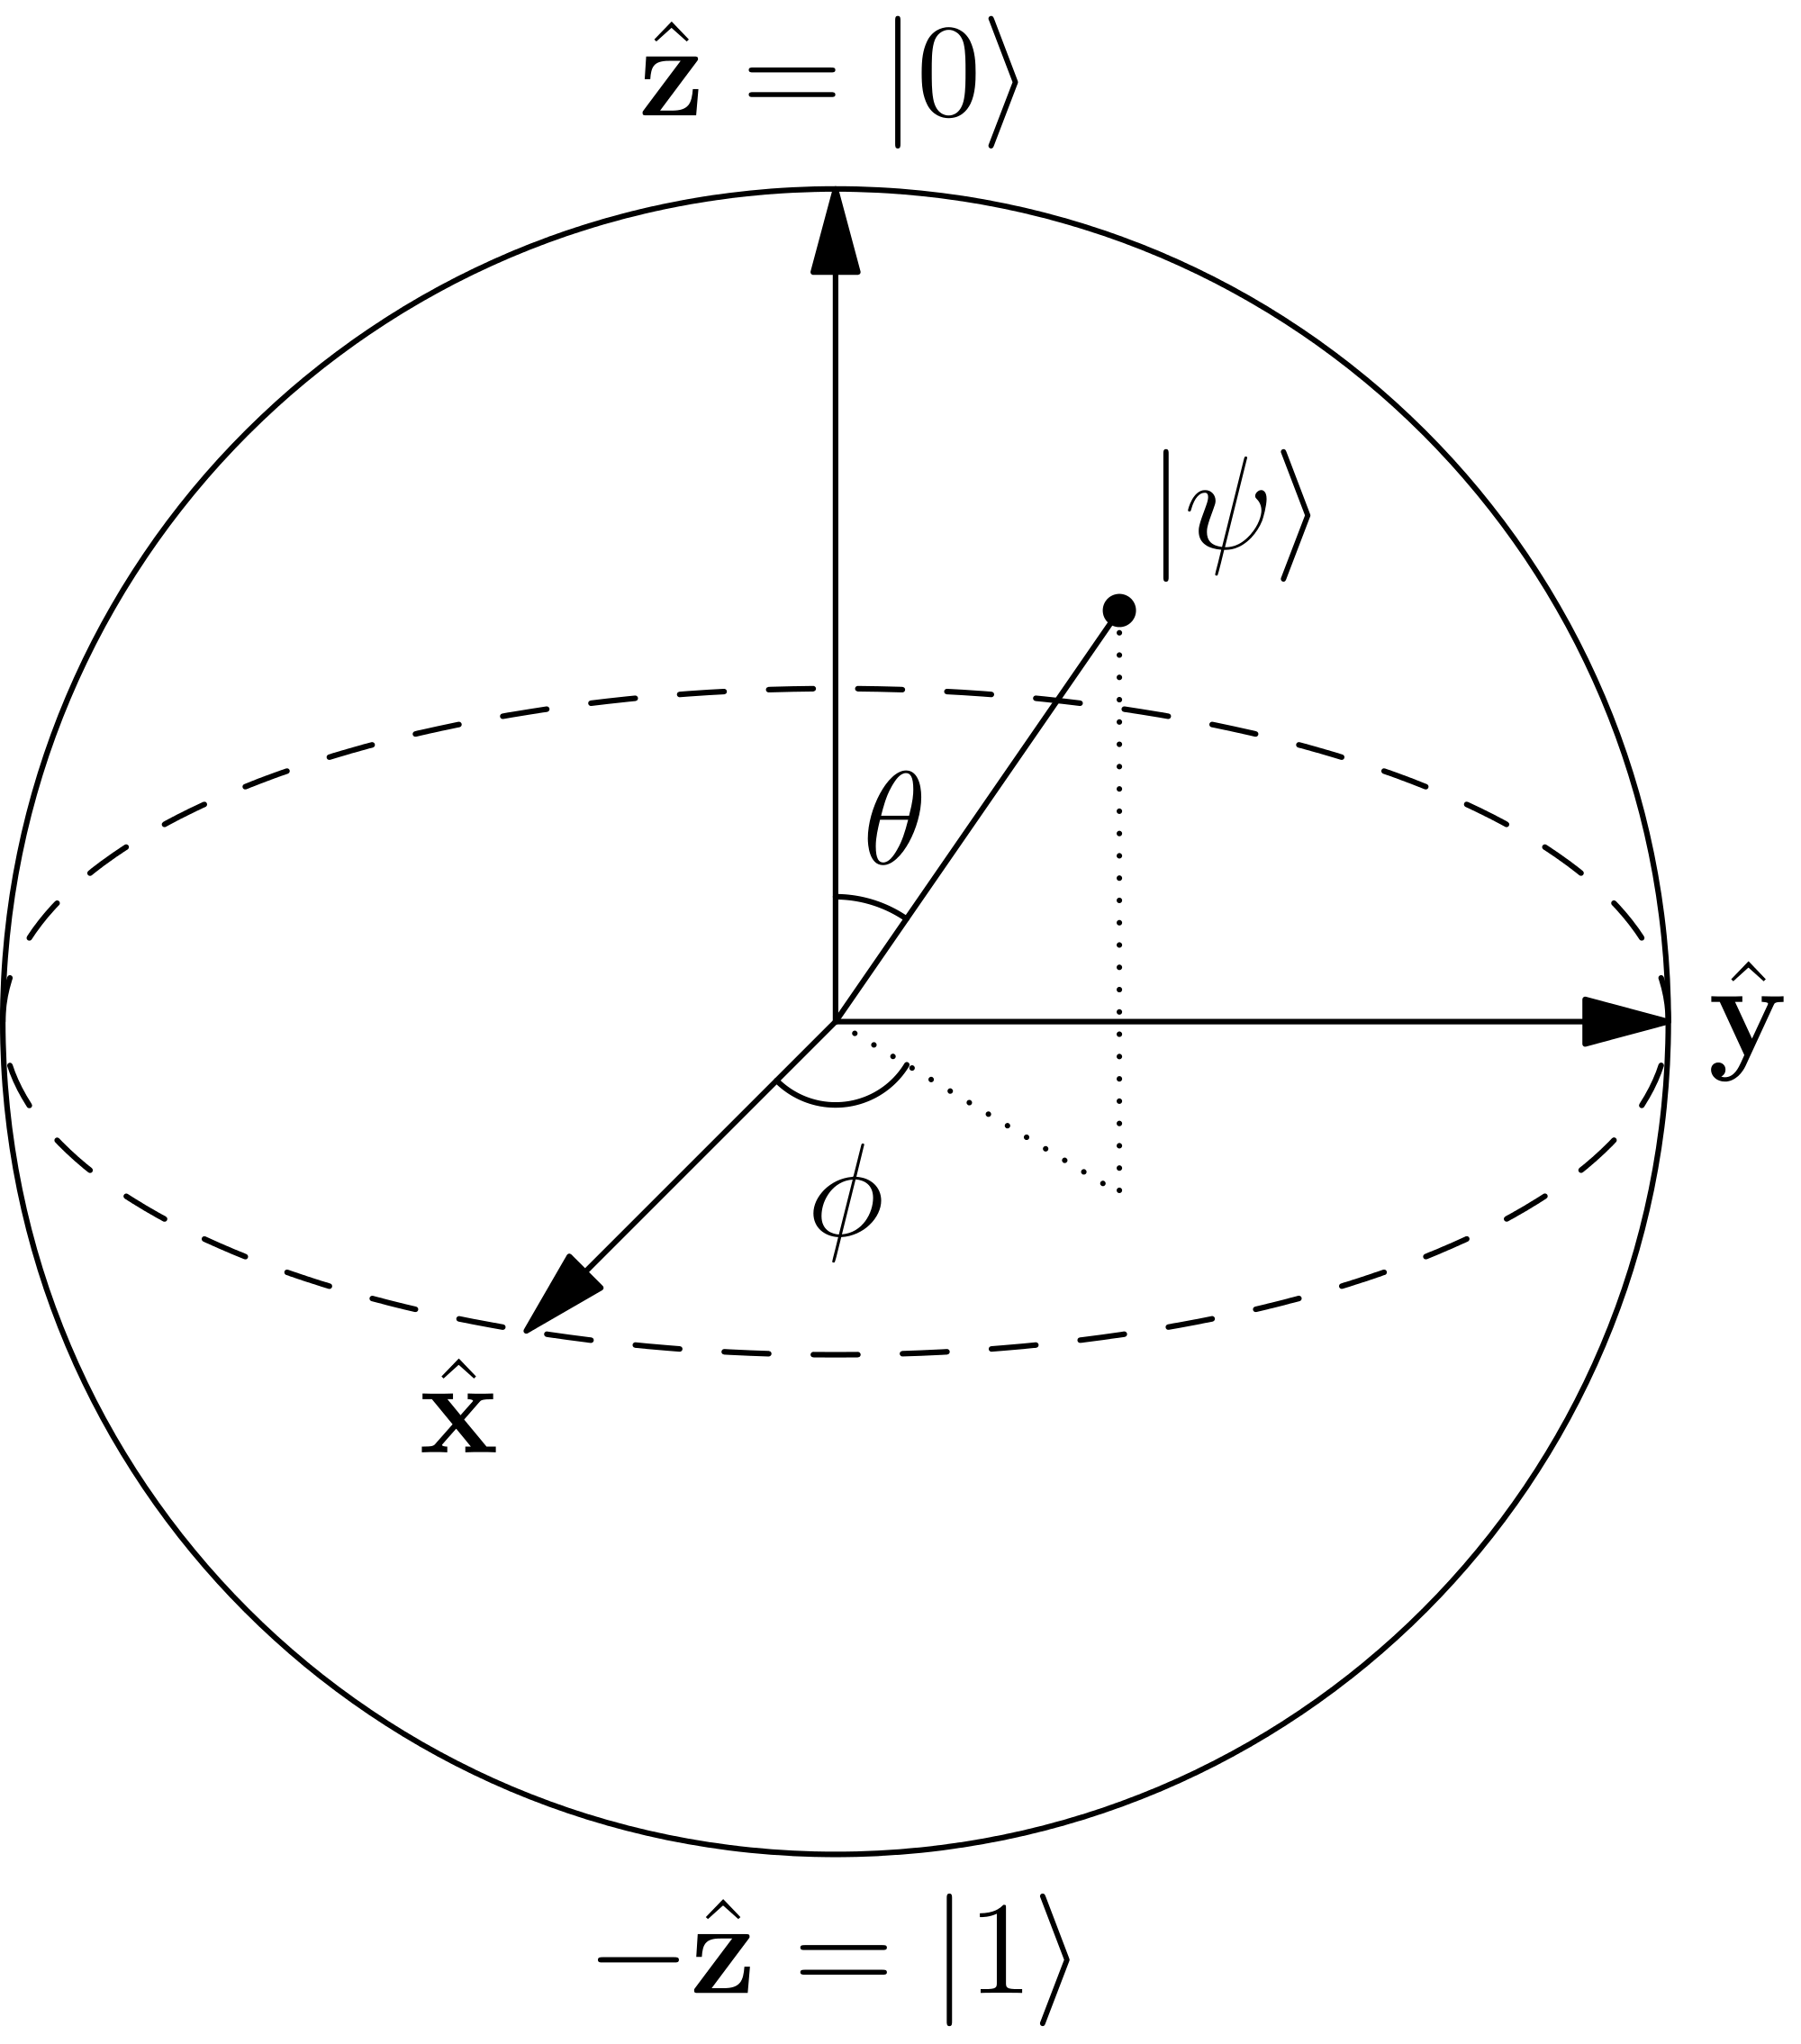
\includegraphics[width=0.8\textwidth]{blochsphere.png}
       \captionsetup{justification=raggedright, singlelinecheck=false}
       \captionof{figure}{\footnotesize{Arbitrary two-dimensional qubit $\ket{\psi}$ visualized on the Bloch sphere.} }
\end{minipage}%%%%%
\begin{minipage}[c][][b]{.5\textwidth}
Most general form of a 2-D qubit:
\begin{equation}
\label{equ: blochqubit}
\ket{q} = \alpha \ket{0} + \beta \ket{1}
\end{equation}
where $\alpha,\beta \in \mathbb{C}$.\\
\\
Can also be visualized in spherical polar coords on the unit or Bloch sphere as follows: 

\begin{equation}
\label{equ: blochqubit}
\ket{q} = \cos\frac{\theta}{2} \ket{0} + e^{i \phi} \sin\frac{\theta}{2} \ket{1}
\end{equation}
where $0 \leq \theta \leq \pi$ and $0 \leq \phi \leq 2\pi$
\null
\par\xdef\tpd{\the\prevdepth}
\end{minipage}


\end{frame}
}

{
\setbeamertemplate{frame footer}{\tiny{\textsuperscript{1}IBM. (2016). What is big data? https://www-01.ibm.com/software/data/bigdata/what-is-big
-data.html. (Accessed: 2016-09-08) \newline
\textsuperscript{2} Bekkerman, R., Bilenko, M., \& Langford, J. (2011). Scaling up machine learning: Parallel and distributed
approaches. Cambridge University Press.}}
\begin{frame}[fragile]{Classical Machine Learning}
   
\begin{itemize}
	\item Approximately 2.5 quintillion (${10}^{18}$) bytes of digital data are created every day\textsuperscript{1}
	\item Need for advanced algorithms that can make sense of data content, retrieve patterns and reveal correlations $\rightarrow$ Machine learning (ML) 
	\item ML algorithms often involve
	\begin{itemize}
	\item solving large systems of linear equations
	\item inverting large matrices
	\item distance computations
	\end{itemize}
	\item Performing these computations on large data
sets gets increasingly difficult\textsuperscript{2}

%when i.e. $\mathcal{O}(input size)$ or $\mathcal{O}(input size^{k})$ for some constant k\textsuperscript{2}
%essentially manipulations on big vectors and matrices

\end{itemize}

\end{frame}
}

{
\setbeamertemplate{frame footer}{}
\begin{frame}[fragile]{Classical Machine Learning}
   
Machine learning can be subdivided into three major fields.

\metroset{block=fill}

\begin{alertblock}{Supervised ML}
- Based on \emph{input} and \emph{output} data\\
\centering{
"I know how to classify this data but I need the algorithm to do the computations for me."}
\end{alertblock}

\begin{exampleblock}{Unsupervised ML}
- Based on \emph{input} data only\\
\centering{
"I have no clue how to classify this data, can the algorithm create a classifier for me?"}
\end{exampleblock}

\begin{block}{Reinforcement learning}
- Based on \emph{input} data only\\
\centering{
"I have no clue how to classify this data, can the algorithm classify this data and I'll give it a reward if it's correct or I'll punish it if it's not."}
\end{block}

\end{frame}
}

{
\setbeamertemplate{frame footer}{}
\begin{frame}[fragile]{Classical Machine Learning}
   
Machine learning can be subdivided into three major fields.$\mathcal{O}(input size)$

\metroset{block=fill}

\begin{alertblock}{Supervised ML}
- Based on \emph{input} and \emph{output} data\\
\centering{
"I know how to classify this data but I need the algorithm to do the computations for me."}
\end{alertblock}

\begin{exampleblock}{\textcolor{gray}{Unsupervised ML}}
\color{gray}
- Based on \emph{input} data only\\
\centering{
"I have no clue how to classify this data, can the algorithm create a classifier for me?"}
\end{exampleblock}

\begin{block}{\textcolor{gray}{Reinforcement learning}}
\color{gray}
- Based on \emph{input} data only\\
\centering{
"I have no clue how to classify this data, can the algorithm classify this data and I'll give it a reward if it's correct or I'll punish it if it's not."}
\end{block}

\end{frame}
}

{
\setbeamertemplate{frame footer}{References go here}
\begin{frame}[fragile]{Quantum Machine Learning}

Some general info about QML. How can quantum computing aid classical machine learning?

\end{frame}
}

{
\setbeamertemplate{frame footer}{References go here}
\begin{frame}[fragile]{Experimental realizations so far}


Until now there have been only few experimental verifications of QML algorithms that establish proof-
of-concept. Li, Liu, Xu, and Du (2015) successfully distinguished a handwritten six from a nine using a
quantum support vector machine on a four-qubit nuclear magnetic resonance test bench. In addition, Cai
et al. (2015) were first to experimentally demonstrate quantum machine learning on a photonic QC and
showed that the distance between two vectors and their inner product can indeed be computed quantum
mechanically. Lastly, Ristè et al. (2015) solved a learning parity problem with five superconducting qubits
and found that a quantum advantage can already be observed in non error-corrected systems.


%Explain the experimental results that have been shown so far. Outline problems with non-error corrected qubits, gate times and small qubit numbers.

%> only proof-of-concept so far
%little is known about full procedure from crude data to final classification

\end{frame}
}

{
\setbeamertemplate{frame footer}{\tiny{\textsuperscript{1}Reprinted from GitHub, Burton de Wilde, Retrieved September 13, 2016, from http://bdewilde.github.io/blog/
blogger/2012/10/26/classification-of-hand-written-digits-3/. Copyright 2012 by Burton de Wilde. Reprinted with
permission.}}
\begin{frame}[fragile]{Classical k-nearest neighbour}
 
 \begin{minipage}[t]{.5\textwidth}
      
Some description goes here.
\end{minipage}%%%%%
\begin{minipage}[c]{.5\textwidth}
%\centering
       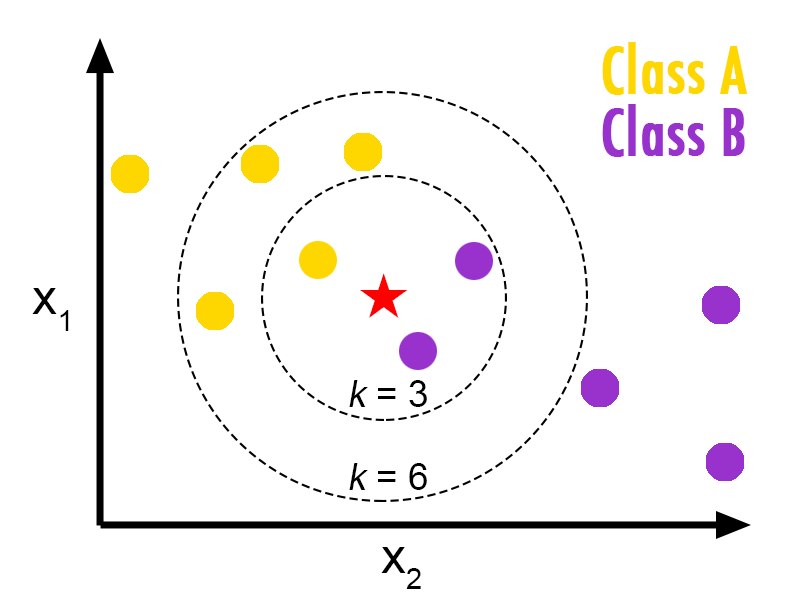
\includegraphics[width=\textwidth]{knn-concept.png}
       \captionsetup{justification=raggedright, singlelinecheck=false}
      \captionof{figure}{\footnotesize{Visualization of a kNN classifier\footnotemark[1]}}

\end{minipage}

 
\end{frame}
}

{
\setbeamertemplate{frame footer}{References go here}
\begin{frame}[fragile]{Quantum k-nearest neighbour}
 
Two different algorithms with respect to initial state preparation:

\begin{alertblock}{Data encoded into qubits}
%speed-up not very clear since the \# of qubits increases linearly with the \# of classical bits
k-dimensional probability vector requires $4k$ classical bits which are encoded one-to-one into $4k$ qubits, e.g.\\
\vspace{2mm}
$\begin{pmatrix}
 \textcolor{blue}{0.6} \\ 
 \textcolor{orange}{0.4}
 \end{pmatrix}*10 \rightarrow \begin{pmatrix}
 \textcolor{blue}{6} \\ 
 \textcolor{orange}{4}
 \end{pmatrix} \rightarrow \begin{pmatrix}
 \textcolor{blue}{0110} \\ 
 \textcolor{orange}{0100}
 \end{pmatrix} \rightarrow n=\textcolor{blue}{0110}\textcolor{orange}{0100} \rightarrow \ket{n} = \ket{\textcolor{blue}{0110}\textcolor{orange}{0100}}$\\
%\textbf{Only slight speed up possible}
\end{alertblock}
\vspace{3mm}
\begin{alertblock}{\textcolor{gray}{Data encoded into amplitudes}}
\textcolor{gray}{k-dimensional probability vector is encoded into $log_{2}(k)$ qubits, e.g.\\ 
\vspace{2mm}
$\begin{pmatrix}
 0.6 \\ 
 0.4
 \end{pmatrix} \quad \rightarrow \quad \ket{n} = \sqrt{0.6}\ket{0}+\sqrt{0.4}\ket{1}$\\
%\textbf{Possibility of exponential speed up}
}
\end{alertblock}

\end{frame}
}

{
\setbeamertemplate{frame footer}{References go here}
\begin{frame}[fragile]{Quantum k-nearest neighbour}
 
Two different algorithms with respect to initial state preparation:

\begin{alertblock}{\textcolor{gray}{Data encoded into qubits}}
%speed-up not very clear since the \# of qubits increases linearly with the \# of classical bits
\textcolor{gray}{k-dimensional probability vector requires $4k$ classical bits which are encoded one-to-one into $4k$ qubits, e.g.\\
\vspace{2mm}
$\begin{pmatrix}
 0.6 \\ 
 0.4
 \end{pmatrix}*10 \rightarrow \begin{pmatrix}
 6 \\ 
 4
 \end{pmatrix} \rightarrow \begin{pmatrix}
 0110 \\ 
 0100
 \end{pmatrix} \rightarrow n=01100100 \rightarrow \ket{n} = \ket{01100100}$\\
%\textbf{Only slight speed up possible}
}
\end{alertblock}  
\vspace{3mm}
\begin{alertblock}{Data encoded into amplitudes}
k-dimensional probability vector is encoded into $log_{2}(k)$ qubits, e.g.\\ 
\vspace{2mm}
$\begin{pmatrix}
 \textcolor{blue}{0.6} \\ 
 \textcolor{orange}{0.4}
 \end{pmatrix} \quad \rightarrow \quad \ket{n} = \sqrt{\textcolor{blue}{0.6}}\ket{0}+\sqrt{\textcolor{orange}{0.4}}\ket{1}$\\
%\textbf{Possibility of exponential speed up}
\end{alertblock}


\end{frame}
}


\section{Amplitude-based kNN algorithm}
{
\setbeamertemplate{frame footer}{References go here}
\begin{frame}{The algorithm}
	\themename supports 4 different titleformats:
	\begin{itemize}
		\item Regular
		\item \textsc{Smallcaps}
		\item \textsc{allsmallcaps}
		\item ALLCAPS
	\end{itemize}
	They can either be set at once for every title type or individually.
	
	\metroset{block=fill}
	\begin{alertblock}{Algorithmic complexity}
	$\mathcal{O}(\frac{1}{p_{acc}})$
	\end{alertblock}
\end{frame}
}

{
\setbeamertemplate{frame footer}{References go here}
\begin{frame}{Implementation with IBM's quantum computer}
	This frame uses the \texttt{smallcaps} titleformat.

	\begin{alertblock}{Potential Problems}
		Be aware, that not every font supports small caps. If for example you typeset your presentation with pdfTeX and the Computer Modern Sans Serif font, every text in smallcaps will be typeset with the Computer Modern Serif font instead.
	\end{alertblock}
\end{frame}
}

{
\setbeamertemplate{frame footer}{References go here}
\begin{frame}{Controlled U gate}
	This frame uses the \texttt{smallcaps} titleformat.

	\begin{alertblock}{Potential Problems}
		Be aware, that not every font supports small caps. If for example you typeset your presentation with pdfTeX and the Computer Modern Sans Serif font, every text in smallcaps will be typeset with the Computer Modern Serif font instead.
	\end{alertblock}
	
	\metroset{block=fill}
	\begin{alertblock}{Algorithmic complexity}
	$\mathcal{O}(\frac{1}{p_{acc}})+\mathcal{O}(somestuff)$
	\end{alertblock}
\end{frame}

}

{
\setbeamertemplate{frame footer}{References go here}
\begin{frame}{Problems with universal gate sets}
	This frame uses the \texttt{allsmallcaps} titleformat.

	\begin{alertblock}{Potential problems}
		As this titleformat also uses smallcaps you face the same problems as with the \texttt{smallcaps} titleformat. Additionally this format can cause some other problems. Please refer to the documentation if you consider using it.
\end{alertblock}

		As a rule of thumb: Just use it for plaintext-only titles.
\metroset{block=fill}
	\begin{alertblock}{Algorithmic complexity}
	$\mathcal{O}(\frac{1}{p_{acc}})+\mathcal{O}(somestuff)+\mathcal{O}(somemorestuff)$
	\end{alertblock}
\end{frame}
}
{
\setbeamertemplate{frame footer}{References go here}
\begin{frame}{All caps}
	This frame uses the \texttt{allcaps} titleformat.

	\begin{alertblock}{Potential Problems}
		This titleformat is not as problematic as the \texttt{allsmallcaps} format, but basically suffers from the same deficiencies. So please have a look at the documentation if you want to use it.
	\end{alertblock}
\end{frame}
}

\section{Qubit-based kNN quantum algorithm}

{
\setbeamertemplate{frame footer}{References go here}
\begin{frame}[fragile]{Typography}
      \begin{verbatim}The theme provides sensible defaults to
\emph{emphasize} text, \alert{accent} parts
or show \textbf{bold} results.\end{verbatim}

  \begin{center}becomes\end{center}

  The theme provides sensible defaults to \emph{emphasize} text,
  \alert{accent} parts or show \textbf{bold} results.
\end{frame}
}

{
\setbeamertemplate{frame footer}{References go here}
\begin{frame}{Font feature test}
  \begin{itemize}
    \item Regular
    \item \textit{Italic}
    \item \textsc{SmallCaps}
    \item \textbf{Bold}
    \item \textbf{\textit{Bold Italic}}
    \item \textbf{\textsc{Bold SmallCaps}}
    \item \texttt{Monospace}
    \item \texttt{\textit{Monospace Italic}}
    \item \texttt{\textbf{Monospace Bold}}
    \item \texttt{\textbf{\textit{Monospace Bold Italic}}}
  \end{itemize}
\end{frame}
}

\begin{frame}{Lists}
  \begin{columns}[T,onlytextwidth]
    \column{0.33\textwidth}
      Items
      \begin{itemize}
        \item Milk \item Eggs \item Potatos
      \end{itemize}

    \column{0.33\textwidth}
      Enumerations
      \begin{enumerate}
        \item First, \item Second and \item Last.
      \end{enumerate}

    \column{0.33\textwidth}
      Descriptions
      \begin{description}
        \item[PowerPoint] Meeh. \item[Beamer] Yeeeha.
      \end{description}
  \end{columns}
\end{frame}
\begin{frame}{Animation}
  \begin{itemize}[<+- | alert@+>]
    \item \alert<4>{This is\only<4>{ really} important}
    \item Now this
    \item And now this
  \end{itemize}
\end{frame}
\begin{frame}{Figures}
  \begin{figure}
    \newcounter{density}
    \setcounter{density}{20}
    \begin{tikzpicture}
      \def\couleur{alerted text.fg}
      \path[coordinate] (0,0)  coordinate(A)
                  ++( 90:5cm) coordinate(B)
                  ++(0:5cm) coordinate(C)
                  ++(-90:5cm) coordinate(D);
      \draw[fill=\couleur!\thedensity] (A) -- (B) -- (C) --(D) -- cycle;
      \foreach \x in {1,...,40}{%
          \pgfmathsetcounter{density}{\thedensity+20}
          \setcounter{density}{\thedensity}
          \path[coordinate] coordinate(X) at (A){};
          \path[coordinate] (A) -- (B) coordinate[pos=.10](A)
                              -- (C) coordinate[pos=.10](B)
                              -- (D) coordinate[pos=.10](C)
                              -- (X) coordinate[pos=.10](D);
          \draw[fill=\couleur!\thedensity] (A)--(B)--(C)-- (D) -- cycle;
      }
    \end{tikzpicture}
    \caption{Rotated square from
    \href{http://www.texample.net/tikz/examples/rotated-polygons/}{texample.net}.}
  \end{figure}
\end{frame}
\begin{frame}{Tables}
  \begin{table}
    \caption{Largest cities in the world (source: Wikipedia)}
    \begin{tabular}{lr}
      \toprule
      City & Population\\
      \midrule
      Mexico City & 20,116,842\\
      Shanghai & 19,210,000\\
      Peking & 15,796,450\\
      Istanbul & 14,160,467\\
      \bottomrule
    \end{tabular}
  \end{table}
\end{frame}
\begin{frame}{Blocks}
  Three different block environments are pre-defined and may be styled with an
  optional background color.

  \begin{columns}[T,onlytextwidth]
    \column{0.5\textwidth}
      \begin{block}{Default}
        Block content.
      \end{block}

      \begin{alertblock}{Alert}
        Block content.
      \end{alertblock}

      \begin{exampleblock}{Example}
        Block content.
      \end{exampleblock}

    \column{0.5\textwidth}

      \metroset{block=fill}

      \begin{block}{Default}
        Block content.
      \end{block}

      \begin{alertblock}{Alert}
        Block content.
      \end{alertblock}

      \begin{exampleblock}{Example}
        Block content.
      \end{exampleblock}

  \end{columns}
\end{frame}
\begin{frame}{Math}
  \begin{equation*}
    e = \lim_{n\to \infty} \left(1 + \frac{1}{n}\right)^n
  \end{equation*}
\end{frame}
\begin{frame}{Line plots}
  \begin{figure}
    \begin{tikzpicture}
      \begin{axis}[
        mlineplot,
        width=0.9\textwidth,
        height=6cm,
      ]

        \addplot {sin(deg(x))};
        \addplot+[samples=100] {sin(deg(2*x))};

      \end{axis}
    \end{tikzpicture}
  \end{figure}
\end{frame}
\begin{frame}{Bar charts}
  \begin{figure}
    \begin{tikzpicture}
      \begin{axis}[
        mbarplot,
        xlabel={Foo},
        ylabel={Bar},
        width=0.9\textwidth,
        height=6cm,
      ]

      \addplot plot coordinates {(1, 20) (2, 25) (3, 22.4) (4, 12.4)};
      \addplot plot coordinates {(1, 18) (2, 24) (3, 23.5) (4, 13.2)};
      \addplot plot coordinates {(1, 10) (2, 19) (3, 25) (4, 15.2)};

      \legend{lorem, ipsum, dolor}

      \end{axis}
    \end{tikzpicture}
  \end{figure}
\end{frame}
\begin{frame}{Quotes}
  \begin{quote}
    Veni, Vidi, Vici
  \end{quote}
\end{frame}

\section{Conclusion}

\begin{frame}{Summary}

sefsefesfsefsef
\end{frame}

\begin{frame}{References}
  Some references to showcase [allowframebreaks] \cite{knuth92,ConcreteMath,Simpson,Er01,greenwade93}
\end{frame}

\begin{frame}[standout]
  Questions?
\end{frame}


\appendix

\begin{frame}[fragile]{Backup slide I}
fefesfesfesfefesf
\end{frame}

\begin{frame}[allowframebreaks]{Backup slide II}

  \bibliography{demo}
  \bibliographystyle{abbrv}

\end{frame}

\end{document}
